\documentclass[border=5pt]{standalone}
\usepackage{tikz}

\begin{document}
		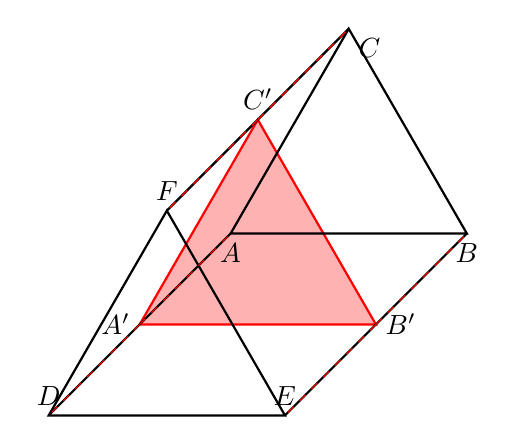
\begin{tikzpicture}
		% Define coordinates
		\coordinate (A) at (0,0);
		\coordinate (B) at (3,0);
		\coordinate (C) at (1.5,2.6);
		\coordinate (D) at (0,0,6);
		\coordinate (E) at (3,0,6);
		\coordinate (F) at (1.5,2.6,6);
		
		% Define horizontal section coordinates (e.g., halfway up the prism)
		\pgfmathsetmacro{\zsection}{3}
		\coordinate (A') at (0,0,\zsection);
		\coordinate (B') at (3,0,\zsection);
		\coordinate (C') at (1.5,2.6,\zsection);
		
		% Draw horizontal section first
		\fill[red!30] (A') -- (B') -- (C') -- cycle;
		\draw[thick, red] (A') -- (B') -- (C') -- cycle;
		
		% Draw base triangle
		\draw[thick] (A) -- (B) -- (C) -- cycle;
		
		% Draw top triangle
		\draw[thick] (D) -- (E) -- (F) -- cycle;
		
		% Draw vertical edges
		\draw[thick] (A) -- (D);
		\draw[thick] (B) -- (E);
		\draw[thick] (C) -- (F);
		
		% Draw projections to the base and top
		\draw[dashed, red] (A') -- (A);
		\draw[dashed, red] (B') -- (B);
		\draw[dashed, red] (C') -- (C);
		\draw[dashed, red] (A') -- (D);
		\draw[dashed, red] (B') -- (E);
		\draw[dashed, red] (C') -- (F);
		
		% Labels for clarity
		\node at (A) [below] {$A$};
		\node at (B) [below] {$B$};
		\node at (C) [below right] {$C$};
		\node at (D) [above] {$D$};
		\node at (E) [above] {$E$};
		\node at (F) [above] {$F$};
		\node at (A') [left] {$A'$};
		\node at (B') [right] {$B'$};
		\node at (C') [above] {$C'$};
		
	\end{tikzpicture}
\end{document}